\documentclass{standalone}
\usepackage{tikz}
\usetikzlibrary{patterns, positioning}


\begin{document}
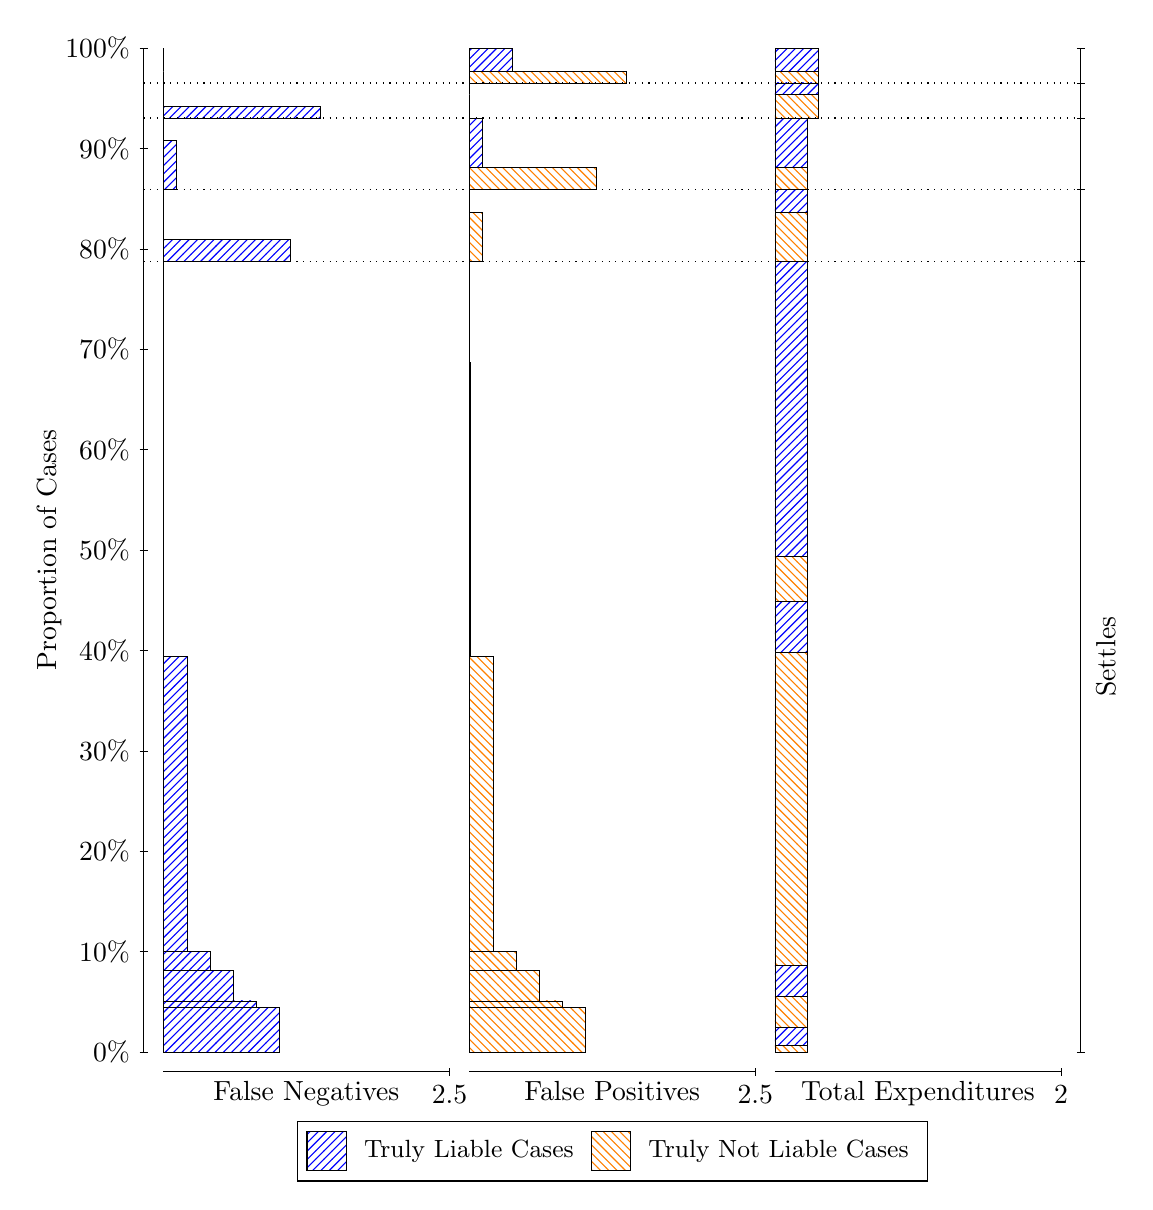
\begin{tikzpicture}
\draw[black, very thin] (1.5,1.75) -- (1.5,14.5);
\node[rotate=90, text=black, anchor=center] at (0.3, 8.125) {Proportion of Cases};
\draw[black, very thin] (1.45,1.75) -- (1.55,1.75);
\node[text=black, anchor=east] at (1.45, 1.75) {0\%};
\draw[black, very thin] (1.45,3.025) -- (1.55,3.025);
\node[text=black, anchor=east] at (1.45, 3.025) {10\%};
\draw[black, very thin] (1.45,4.3) -- (1.55,4.3);
\node[text=black, anchor=east] at (1.45, 4.3) {20\%};
\draw[black, very thin] (1.45,5.575) -- (1.55,5.575);
\node[text=black, anchor=east] at (1.45, 5.575) {30\%};
\draw[black, very thin] (1.45,6.85) -- (1.55,6.85);
\node[text=black, anchor=east] at (1.45, 6.85) {40\%};
\draw[black, very thin] (1.45,8.125) -- (1.55,8.125);
\node[text=black, anchor=east] at (1.45, 8.125) {50\%};
\draw[black, very thin] (1.45,9.4) -- (1.55,9.4);
\node[text=black, anchor=east] at (1.45, 9.4) {60\%};
\draw[black, very thin] (1.45,10.675) -- (1.55,10.675);
\node[text=black, anchor=east] at (1.45, 10.675) {70\%};
\draw[black, very thin] (1.45,11.95) -- (1.55,11.95);
\node[text=black, anchor=east] at (1.45, 11.95) {80\%};
\draw[black, very thin] (1.45,13.225) -- (1.55,13.225);
\node[text=black, anchor=east] at (1.45, 13.225) {90\%};
\draw[black, very thin] (1.45,14.5) -- (1.55,14.5);
\node[text=black, anchor=east] at (1.45, 14.5) {100\%};

\draw[black, very thin] (13.4,1.75) -- (13.4,14.5);
\draw[black, very thin] (13.35,1.75) -- (13.45,1.75);
\node[anchor=west] at (13.35, 1.75) {};
\draw[black, very thin] (13.35,11.789) -- (13.45,11.789);
\node[anchor=west] at (13.35, 11.789) {};
\draw[black, very thin] (13.35,12.7) -- (13.45,12.7);
\node[anchor=west] at (13.35, 12.7) {};
\draw[black, very thin] (13.35,13.611) -- (13.45,13.611);
\node[anchor=west] at (13.35, 13.611) {};
\draw[black, very thin] (13.35,14.056) -- (13.45,14.056);
\node[anchor=west] at (13.35, 14.056) {};
\draw[black, very thin] (13.35,14.5) -- (13.45,14.5);
\node[anchor=west] at (13.35, 14.5) {};

\draw[black, very thin, pattern color=blue, pattern=north east lines] (1.75,1.75) rectangle (3.2215,2.3164);
\draw[black, very thin, pattern color=blue, pattern=north east lines] (1.75,2.3164) rectangle (2.9308,2.3986);
\draw[black, very thin, pattern color=blue, pattern=north east lines] (1.75,2.3986) rectangle (2.6402,2.7895);
\draw[black, very thin, pattern color=blue, pattern=north east lines] (1.75,2.7895) rectangle (2.3495,3.0237);
\draw[black, very thin, pattern color=blue, pattern=north east lines] (1.75,3.0237) rectangle (2.0588,6.7693);
\draw[black, very thin, pattern color=orange, pattern=north west lines] (1.75,6.7693) rectangle (1.75,11.789);
\draw[black, very thin, pattern color=blue, pattern=north east lines] (1.75,11.789) rectangle (3.3668,12.074);
\draw[black, very thin, pattern color=orange, pattern=north west lines] (1.75,12.074) rectangle (1.75,12.7);
\draw[black, very thin, pattern color=blue, pattern=north east lines] (1.75,12.7) rectangle (1.9135,13.326);
\draw[black, very thin, pattern color=orange, pattern=north west lines] (1.75,13.326) rectangle (1.75,13.611);
\draw[black, very thin, pattern color=blue, pattern=north east lines] (1.75,13.611) rectangle (3.7483,13.755);
\draw[black, very thin, pattern color=orange, pattern=north west lines] (1.75,13.755) rectangle (1.75,14.056);
\draw[black, very thin, pattern color=orange, pattern=north west lines] (1.75,14.056) rectangle (1.75,14.199);
\draw[black, very thin, pattern color=blue, pattern=north east lines] (1.75,14.199) rectangle (1.75,14.5);
\draw[black, very thin, pattern color=orange, pattern=north west lines] (5.6333,1.75) rectangle (7.1048,2.3164);
\draw[black, very thin, pattern color=orange, pattern=north west lines] (5.6333,2.3164) rectangle (6.8142,2.3985);
\draw[black, very thin, pattern color=orange, pattern=north west lines] (5.6333,2.3985) rectangle (6.5235,2.7894);
\draw[black, very thin, pattern color=orange, pattern=north west lines] (5.6333,2.7894) rectangle (6.2328,3.0237);
\draw[black, very thin, pattern color=orange, pattern=north west lines] (5.6333,3.0237) rectangle (5.9422,6.7694);
\draw[black, very thin, pattern color=blue, pattern=north east lines] (5.6333,6.7694) rectangle (5.6515,10.515);
\draw[black, very thin, pattern color=blue, pattern=north east lines] (5.6333,10.515) rectangle (5.6333,11.789);
\draw[black, very thin, pattern color=orange, pattern=north west lines] (5.6333,11.789) rectangle (5.7968,12.414);
\draw[black, very thin, pattern color=blue, pattern=north east lines] (5.6333,12.414) rectangle (5.6333,12.7);
\draw[black, very thin, pattern color=orange, pattern=north west lines] (5.6333,12.7) rectangle (7.2502,12.985);
\draw[black, very thin, pattern color=blue, pattern=north east lines] (5.6333,12.985) rectangle (5.7968,13.611);
\draw[black, very thin, pattern color=orange, pattern=north west lines] (5.6333,13.611) rectangle (5.6333,13.912);
\draw[black, very thin, pattern color=blue, pattern=north east lines] (5.6333,13.912) rectangle (5.6333,14.056);
\draw[black, very thin, pattern color=orange, pattern=north west lines] (5.6333,14.056) rectangle (7.6317,14.199);
\draw[black, very thin, pattern color=blue, pattern=north east lines] (5.6333,14.199) rectangle (6.1783,14.5);
\draw[black, very thin, pattern color=orange, pattern=north west lines] (9.5167,1.75) rectangle (9.9254,1.8322);
\draw[black, very thin, pattern color=blue, pattern=north east lines] (9.5167,1.8322) rectangle (9.9254,2.0664);
\draw[black, very thin, pattern color=orange, pattern=north west lines] (9.5167,2.0664) rectangle (9.9254,2.4573);
\draw[black, very thin, pattern color=blue, pattern=north east lines] (9.5167,2.4573) rectangle (9.9254,2.8482);
\draw[black, very thin, pattern color=orange, pattern=north west lines] (9.5167,2.8482) rectangle (9.9254,6.8282);
\draw[black, very thin, pattern color=blue, pattern=north east lines] (9.5167,6.8282) rectangle (9.9254,7.4768);
\draw[black, very thin, pattern color=orange, pattern=north west lines] (9.5167,7.4768) rectangle (9.9254,8.0431);
\draw[black, very thin, pattern color=blue, pattern=north east lines] (9.5167,8.0431) rectangle (9.9254,11.789);
\draw[black, very thin, pattern color=orange, pattern=north west lines] (9.5167,11.789) rectangle (9.9254,12.414);
\draw[black, very thin, pattern color=blue, pattern=north east lines] (9.5167,12.414) rectangle (9.9254,12.7);
\draw[black, very thin, pattern color=orange, pattern=north west lines] (9.5167,12.7) rectangle (9.9254,12.985);
\draw[black, very thin, pattern color=blue, pattern=north east lines] (9.5167,12.985) rectangle (9.9254,13.611);
\draw[black, very thin, pattern color=orange, pattern=north west lines] (9.5167,13.611) rectangle (10.062,13.912);
\draw[black, very thin, pattern color=blue, pattern=north east lines] (9.5167,13.912) rectangle (10.062,14.056);
\draw[black, very thin, pattern color=orange, pattern=north west lines] (9.5167,14.056) rectangle (10.062,14.199);
\draw[black, very thin, pattern color=blue, pattern=north east lines] (9.5167,14.199) rectangle (10.062,14.5);
\draw[black, dotted] (1.5,11.789) -- (13.4,11.789);
\draw[black, dotted] (1.5,12.7) -- (13.4,12.7);
\draw[black, dotted] (1.5,13.611) -- (13.4,13.611);
\draw[black, dotted] (1.5,14.056) -- (13.4,14.056);
\draw[black, very thin] (1.75,1.5) -- (5.3833,1.5);
\node[text=black, anchor=north] at (3.5667, 1.5) {False Negatives};
\draw[black, very thin] (5.3833,1.45) -- (5.3833,1.55);
\node[text=black, anchor=north] at (5.3833, 1.45) {2.5};

\draw[black, very thin] (5.6333,1.5) -- (9.2667,1.5);
\node[text=black, anchor=north] at (7.45, 1.5) {False Positives};
\draw[black, very thin] (9.2667,1.45) -- (9.2667,1.55);
\node[text=black, anchor=north] at (9.2667, 1.45) {2.5};

\draw[black, very thin] (9.5167,1.5) -- (13.15,1.5);
\node[text=black, anchor=north] at (11.333, 1.5) {Total Expenditures};
\draw[black, very thin] (13.15,1.45) -- (13.15,1.55);
\node[text=black, anchor=north] at (13.15, 1.45) {2};

\node[text=black, centered, rotate=90] at (13.72, 6.7693) {Settles};





\draw (7.449999999999999,1.5) node[draw=none] (baseCoordinate) {};
\begin{scope}[align=center]
        \matrix[scale=0.5, draw=black, below=0.5cm of baseCoordinate, nodes={draw}, column sep=0.1cm]{
            \node[rectangle, draw, minimum width=0.5cm, minimum height=0.5cm, pattern color=blue, pattern=north east lines] {}; &
            \node[draw=none, font=\small, text=black] (B) {Truly Liable Cases}; &
            \node[rectangle, draw, minimum width=0.5cm, minimum height=0.5cm, pattern color=orange, pattern=north west lines] {}; &
            \node[draw=none, font=\small, text=black] (B) {Truly Not Liable Cases}; \\
            };
\end{scope}

\end{tikzpicture}
\end{document}